\documentclass[aspectratio=169,10pt]{beamer}

% =====================================================================
% GOI TIENG VIET VA FONT
% =====================================================================
\usepackage[T5]{fontenc}
\usepackage[utf8]{inputenc}
\usepackage[vietnamese]{babel}
\usepackage{amsmath,amssymb}
\usepackage{booktabs}
\usepackage{multirow}
\usepackage{tikz}
\usetikzlibrary{arrows.meta,positioning,shapes.geometric,fit,calc}
\usepackage{graphicx}
\usepackage{microtype}

% =====================================================================
% BEAMER THEME & COLOR PALETTE
% =====================================================================
\usetheme{Madrid}
\usecolortheme{whale}

% Mau sac chu dao hien dai
\definecolor{NavyMain}{RGB}{15, 32, 67}       % #0F2043
\definecolor{BlueAccent}{RGB}{30, 58, 138}    % #1E3A8A
\definecolor{EmeraldGreen}{RGB}{5, 150, 105}  % #059669
\definecolor{CrimsonRed}{RGB}{220, 38, 38}    % #DC2626
\definecolor{AmberGold}{RGB}{217, 119, 6}     % #D97706
\definecolor{SlateBg}{RGB}{248, 250, 252}     % #F8FAFC
\definecolor{LightBlueBg}{RGB}{239, 246, 255} % #EFF6FF
\definecolor{LightRedBg}{RGB}{254, 242, 242}  % #FEF2F2

% Ap dung mau cho Beamer
\setbeamercolor{palette primary}{bg=NavyMain,fg=white}
\setbeamercolor{palette secondary}{bg=BlueAccent,fg=white}
\setbeamercolor{palette tertiary}{bg=NavyMain!90!black,fg=white}
\setbeamercolor{structure}{fg=BlueAccent}
\setbeamercolor{title}{bg=NavyMain,fg=white}
\setbeamercolor{frametitle}{bg=NavyMain,fg=white}
\setbeamercolor{block title}{bg=BlueAccent!15,fg=BlueAccent}
\setbeamercolor{block body}{bg=SlateBg,fg=black}
\setbeamercolor{block title alerted}{bg=CrimsonRed!15,fg=CrimsonRed}
\setbeamercolor{block body alerted}{bg=LightRedBg,fg=black}
\setbeamercolor{block title example}{bg=EmeraldGreen!15,fg=EmeraldGreen}
\setbeamercolor{block body example}{bg=EmeraldGreen!5,fg=black}

% Xoa nut dieu huong ruom ra
\setbeamertemplate{navigation symbols}{}

% Footer hien dai
\setbeamertemplate{footline}{
  \leavevmode%
  \hbox{%
  \begin{beamercolorbox}[wd=.333333\paperwidth,ht=2.25ex,dp=1ex,center]{author in head/foot}%
    \usebeamerfont{author in head/foot}Nhóm sinh viên thực hiện
  \end{beamercolorbox}%
  \begin{beamercolorbox}[wd=.333333\paperwidth,ht=2.25ex,dp=1ex,center]{title in head/foot}%
    \usebeamerfont{title in head/foot}Đánh giá hệ đa tác tử LLM
  \end{beamercolorbox}%
  \begin{beamercolorbox}[wd=.333333\paperwidth,ht=2.25ex,dp=1ex,right]{date in head/foot}%
    \usebeamerfont{date in head/foot}\insertframenumber{} / \inserttotalframenumber\hspace*{2ex}
  \end{beamercolorbox}}%
  \vskip0pt%
}

% Dinh nghia macro toan hoc
\newcommand{\dceil}{\Delta_{\mathrm{tran}}}
\newcommand{\dhonest}{\Delta_{\mathrm{thuc}}}
\newcommand{\acc}{\mathrm{acc}}

% =====================================================================
% THONG TIN BIA
% =====================================================================
\title[\textbf{Đánh giá hệ đa tác tử LLM}]{\textbf{\Large ĐÁNH GIÁ LẠI GIÁ TRỊ THỰC CỦA HỆ ĐA TÁC TỬ LLM}}
\subtitle{\large Phân tích cơ chế tương tác và luồng thông tin dưới ba phép kiểm soát}
\author[INT3406]{\textbf{Sinh viên thực hiện:}\\[2pt]
Dương Trọng Nguyên (24022420) \quad Trương Đình Đức (24021419)\\[2pt]
Trần Tùng Dương (24022309) \quad Lê Hoàng Quân (24022433)}
\institute[UET-VNU]{\textbf{Môn học:} Xử lý ngôn ngữ tự nhiên (INT3406)\\[2pt]
\textbf{Giảng viên hướng dẫn:} TS. Trần Hồng Việt\\[3pt]
\textit{Viện Trí tuệ Nhân tạo --- Trường Đại học Công nghệ, ĐHQGHN}}
\date{Tháng 08, 2026}

\begin{document}

% ---------------------------------------------------------------------
% SLIDE 1: TRANG BIA
% ---------------------------------------------------------------------
\begin{frame}[plain]
  \begin{tikzpicture}[remember picture,overlay]
    \node[anchor=north west, xshift=1cm, yshift=-0.8cm] at (current page.north west) {
      
\includegraphics[height=1.2cm]{figs/logo_uet.png}
    };
    \node[anchor=north east, xshift=-1cm, yshift=-0.8cm, align=right] at (current page.north east) {
      \scriptsize\textbf{TRƯỜNG ĐẠI HỌC CÔNG NGHỆ --- ĐHQGHN}\\
      \scriptsize\textbf{VIỆN TRÍ TUỆ NHÂN TẠO}
    };
  \end{tikzpicture}
  \vspace{0.8cm}
  \titlepage
\end{frame}

% ---------------------------------------------------------------------
% SLIDE 2: MUC LUC
% ---------------------------------------------------------------------
\begin{frame}{Nội dung bài thuyết trình}
  \begin{columns}[t]
    \begin{column}{0.48\textwidth}
      \begin{block}{\textbf{Khung lý thuyết \& Phương pháp}}
        \begin{enumerate}
          \item[\textbf{I.}] \textbf{Đặt vấn đề \& Khung định nghĩa}
          \begin{itemize}\footnotesize
            \item Kỳ vọng lý thuyết vs Thực tế thực nghiệm
            \item Hệ ký hiệu cốt lõi ($W, I, E$)
          \end{itemize}
          \item[\textbf{II.}] \textbf{Ba phép kiểm soát phương pháp luận}
          \begin{itemize}\footnotesize
            \item Ngân sách tính toán, Mốc đối chứng, Mẫu số
          \end{itemize}
          \item[\textbf{III.}] \textbf{Tương tác Artifact \& Bóc tách cơ chế}
          \begin{itemize}\footnotesize
            \item Tổn thất do tiếp xúc artifact sai
            \item Kênh truyền dẫn vs Sửa lỗi suy luận
          \end{itemize}
        \end{enumerate}
      \end{block}
    \end{column}
    
    \begin{column}{0.48\textwidth}
      \begin{block}{\textbf{Thực nghiệm \& Ứng dụng thực tế}}
        \begin{enumerate}
          \item[\textbf{IV.}] \textbf{Đóng góp vai trò \& Huấn luyện RL}
          \begin{itemize}\footnotesize
            \item Phân rã giá trị Shapley (16 liên minh)
            \item Năng lực Verifier \& Lối tắt hàm thưởng
          \end{itemize}
          \item[\textbf{V.}] \textbf{Cơ chế mốc tham chiếu \& Thiết kế}
          \begin{itemize}\footnotesize
            \item Điểm đổi dấu $g^* \approx 0{,}09$
            \item Ma trận khuyến nghị kiến trúc
          \end{itemize}
          \item[\textbf{VI.}] \textbf{Hạn chế \& Tiềm năng phát triển}
          \begin{itemize}\footnotesize
            \item Giới hạn quy mô, Hướng phát triển Hybrid
          \end{itemize}
        \end{enumerate}
      \end{block}
    \end{column}
  \end{columns}
\end{frame}

% =====================================================================
% PHAN I: DAT VAN DE & KHUNG DINH NGHIA
% =====================================================================
\section{Phần I: Đặt vấn đề \& Khung định nghĩa}

\begin{frame}{1.1. Đặt vấn đề: Kỳ vọng lý thuyết vs Thực tế thực nghiệm}
  \begin{columns}[c]
    \begin{column}{0.52\textwidth}
      \begin{block}{\textbf{Kỳ vọng phổ biến về Multi-Agent LLM}}
        \begin{itemize}\small
          \item Chia nhỏ quy trình: \textbf{Planner} $\to$ \textbf{Solver} $\to$ \textbf{Verifier} $\to$ \textbf{Aggregator}.
          \item Trực giác: \emph{Nhiều mô hình cùng kiểm tra chéo sẽ phát hiện lỗi tốt hơn một mô hình đơn lẻ.}
          \item Phần lớn bài báo công bố mức tăng biểu kiến từ $+5\%$ đến $+15\%$.
        \end{itemize}
      \end{block}
      
      \begin{alertblock}{\textbf{Hiện tượng thực nghiệm bất thường}}
        \begin{itemize}\small
          \item Trên tập MATH: Mô hình mạnh (7B) tự giải đúng \textbf{46,4\%}.
          \item Khi kèm thêm lời giải \textbf{sai} của mô hình yếu (1.5B), độ chính xác của 7B tụt xuống chỉ còn \textbf{19,2\%} (giảm $-27{,}2$ điểm!).
        \end{itemize}
      \end{alertblock}
    \end{column}
    
    \begin{column}{0.45\textwidth}
      \begin{exampleblock}{\textbf{Câu hỏi nghiên cứu cốt lõi}}
        \centering\vspace{4pt}
        \textit{Khi nào phối hợp đa tác tử thực sự tạo ra giá trị gia tăng, và khi nào nó chỉ là ảo ảnh của việc chọn sai mốc đối chứng?}
        \vspace{4pt}
      \end{exampleblock}
      
      \begin{block}{\textbf{Phạm vi khảo sát}}
        \begin{itemize}\footnotesize
          \item 4 benchmarks: GSM8K, MATH-500, MBPP, HumanEval.
          \item Dải mô hình: 1,5B đến 32B tham số (Qwen, Llama, DeepSeek-Coder).
          \item Môi trường phần cứng: RTX 5090 \& Kaggle T4.
        \end{itemize}
      \end{block}
    \end{column}
  \end{columns}
\end{frame}

\begin{frame}{1.2. Hệ ký hiệu \& Khung phân tích 3 câu hỏi cơ chế}
  \begin{columns}[t]
    \begin{column}{0.48\textwidth}
      \begin{block}{\textbf{1. Ba trạng thái mô hình}}
        \begin{itemize}\footnotesize
          \item \textbf{$W$ (Weak model):} Mô hình yếu tự giải bài $\to$ sinh ra \textbf{artifact} (lời giải).
          \item \textbf{$I$ (Independent strong model):} Mô hình mạnh giải độc lập, không nhìn bài ai.
          \item \textbf{$E$ (Exposed strong model):} Cùng mô hình mạnh, cùng prompt, nhưng ngữ cảnh kèm artifact của $W$.
        \end{itemize}
      \end{block}
      
      \begin{exampleblock}{\textbf{2. Đại lượng đo lường cốt lõi}}
        \begin{itemize}\footnotesize
          \item \textbf{Hiệu quả triển khai thực tế:} $\dhonest = \acc(E) - \acc(I)$
          \item \textbf{Mức cải thiện tối đa (Trần lý tưởng):} $\dceil = G - L + R$
        \end{itemize}
      \end{exampleblock}
    \end{column}
    
    \begin{column}{0.48\textwidth}
      \begin{block}{\textbf{3. Khung 3 câu hỏi cơ chế}}
        \begin{itemize}\footnotesize
          \item \textbf{Cơ hội cải thiện ($G$):}
          $$P(W \text{ đúng} \wedge I \text{ sai})$$
          \textit{Mô hình yếu có giải được bài mà mô hình mạnh bỏ lỡ?}
          
          \item \textbf{Tổn thất tương tác ($L$):}
          $$P(W \text{ sai} \wedge I \text{ đúng} \wedge E \text{ sai})$$
          \textit{Mô hình mạnh có bị làm hỏng bài nó vốn tự làm đúng?}
          
          \item \textbf{Khả năng khai thác ($\kappa$):}
          \textit{Bộ chọn có nhặt đúng lời giải chính xác trong tập ứng viên?}
        \end{itemize}
      \end{block}
    \end{column}
  \end{columns}
\end{frame}

% =====================================================================
% PHAN II: BA PHEP KIEM SOAT PHUONG PHAP LUAN
% =====================================================================
\section{Phần II: Ba phép kiểm soát phương pháp luận}

\begin{frame}{2.1. Vì sao y văn hiện tại thường kết luận sai lệch?}
  \begin{columns}[c]
    \begin{column}{0.32\textwidth}
      \begin{alertblock}{\textbf{1. Chi phí tính toán}}
        \small
        So sánh một pipeline 4 vai (tốn gấp $3\times - 6\times$ token) với 1 mô hình nhỏ chạy 1 lần.
        \vspace{4pt}
        
        $\implies$ \textit{So sánh bất bình đẳng về ngân sách tính toán (FLOPs).}
      \end{alertblock}
    \end{column}
    
    \begin{column}{0.32\textwidth}
      \begin{alertblock}{\textbf{2. Mốc đối chứng}}
        \small
        Đo mức tăng so với mô hình yếu $W$ (mô hình bị sửa) thay vì so với mô hình mạnh $I$.
        \vspace{4pt}
        
        $\implies$ \textit{Thực tế người dùng muốn biết: Gọi thẳng $I$ hay chạy multi-agent?}
      \end{alertblock}
    \end{column}
    
    \begin{column}{0.32\textwidth}
      \begin{alertblock}{\textbf{3. Pha loãng mẫu số}}
        \small
        Tính trung bình trên cả các câu quá dễ (mọi model đều đúng) hoặc quá khó (mọi model đều sai).
        \vspace{4pt}
        
        $\implies$ \textit{Pha loãng và che lấp hiệu ứng can thiệp thực tế.}
      \end{alertblock}
    \end{column}
  \end{columns}
  
  \vspace{8pt}
  \begin{block}{\textbf{Hệ quả phương pháp luận}}
    \centering\small
    Thiếu kiểm soát chi phí và mốc so sánh sẽ \textbf{thổi phồng} hiệu quả; thiếu kiểm soát mẫu số sẽ \textbf{đánh giá thấp} can thiệp.\\
    \textbf{Giải pháp:} Bắt buộc phải áp dụng đồng thời cả 3 phép kiểm soát cùng lúc.
  \end{block}
\end{frame}

\begin{frame}{2.2. Thiết lập 3 phép kiểm soát đối chứng công bằng}
  \begin{columns}[t]
    \begin{column}{0.32\textwidth}
      \begin{block}{\textbf{1. Kiểm soát Compute}}
        \begin{itemize}\footnotesize
          \item Quy đổi FLOPs theo số tham số: Model 7B tốn $\sim 4{,}8\times$ FLOPs so với 1.5B.
          \item Pipeline 4 vai sinh lượng token gấp $2{,}9\times$ (GSM8K) đến $6{,}6\times$ (MATH).
          \item Đối chứng: So sánh ở \textbf{cùng tổng ngân sách FLOPs}.
        \end{itemize}
      \end{block}
    \end{column}
    
    \begin{column}{0.32\textwidth}
      \begin{block}{\textbf{2. Kiểm soát Baseline}}
        \begin{itemize}\footnotesize
          \item Đo đồng thời 2 mốc:
            \begin{itemize}\scriptsize
              \item $\Delta_W = \acc(\text{Hệ}) - \acc(W)$
              \item $\dhonest = \acc(\text{Hệ}) - \acc(I)$
            \end{itemize}
          \item Khẳng định giá trị thực: Chỉ khi $\dhonest > 0$ thì hệ thống mới có giá trị triển khai.
        \end{itemize}
      \end{block}
    \end{column}
    
    \begin{column}{0.32\textwidth}
      \begin{block}{\textbf{3. Kiểm soát Mẫu số}}
        \begin{itemize}\footnotesize
          \item Phân tầng tập dữ liệu MATH:
            \begin{itemize}\scriptsize
              \item $32\%$ bài: Tất cả lượt sinh đều sai.
              \item $25\%$ bài: Tất cả lượt sinh đều đúng.
            \end{itemize}
          \item $57\%$ số câu nằm ngoài khả năng can thiệp $\implies$ Phân tích riêng trên tập bài có biến thiên.
        \end{itemize}
      \end{block}
    \end{column}
  \end{columns}
  
  \vspace{6pt}
  \begin{exampleblock}{\textbf{Quy trình tiền đăng ký \& Kiểm soát sai số}}
    \centering\footnotesize
    Thực hiện 5-fold cross-validation, khóa trước giả thuyết và điều kiện dừng (VOID 16/32 lần chạy không đạt chuẩn kỹ thuật).
  \end{exampleblock}
\end{frame}

% =====================================================================
% PHAN III: HIEN TUONG TUONG TAC ARTIFACT & BOC TACH CO CHE
% =====================================================================
\section{Phần III: Tương tác Artifact \& Bóc tách cơ chế}

\begin{frame}{3.1. Thí nghiệm tác động của Artifact (Artifact Exposure)}
  \begin{columns}[c]
    \begin{column}{0.55\textwidth}
      \begin{tikzpicture}[scale=0.85, transform shape,
        box/.style={draw=BlueAccent, fill=white, rounded corners=3pt, align=center, font=\footnotesize, inner sep=4pt, minimum width=3.8cm},
        arr/.style={-{Stealth[length=2.2mm]}, thick, color=NavyMain}]
        
        \node[box, fill=SlateBg] (q) at (0,0) {\textbf{261 Bài toán MATH}\\(Tập con: Model yếu $W$ giải \textbf{SAI})};
        
        \node[box] (i) at (-2.3,-1.5) {\textbf{Nhánh $I$ (Độc lập)}\\Model mạnh tự giải};
        \node[box, draw=CrimsonRed, fill=LightRedBg] (e) at (2.3,-1.5) {\textbf{Nhánh $E$ (Tiếp xúc)}\\Model mạnh + bài sai của $W$};
        
        \node[box, fill=EmeraldGreen!10, draw=EmeraldGreen] (ri) at (-2.3,-3.0) {Chính xác: \textbf{46,4\%}};
        \node[box, fill=CrimsonRed!15, draw=CrimsonRed] (re) at (2.3,-3.0) {Chính xác: \textbf{19,2\%}};
        
        \draw[arr] (q) -- (i);
        \draw[arr] (q) -- (e);
        \draw[arr] (i) -- (ri);
        \draw[arr] (e) -- (re);
        
        \node[draw=CrimsonRed, fill=white, rounded corners=2pt, font=\scriptsize\bfseries, text=CrimsonRed] at (0,-2.3) {Tụt $-27{,}2$ điểm!};
      \end{tikzpicture}
    \end{column}
    
    \begin{column}{0.42\textwidth}
      \begin{alertblock}{\textbf{Kết quả thực nghiệm}}
        \begin{itemize}\small
          \item Model mạnh bị dẫn dắt sai trên chính những bài nó vốn tự giải quyết được.
          \item Mức giảm: \textbf{$-27{,}2$ điểm} ($p \approx 0$).
        \end{itemize}
      \end{alertblock}
      
      \begin{block}{\textbf{Hiệu ứng hai mặt}}
        \begin{itemize}\small
          \item Kèm bài \textbf{đúng} của $W$: Model mạnh tăng nhẹ ($+1{,}8$ điểm).
          \item Kèm bài \textbf{sai} của $W$: Model mạnh tụt sâu ($-27{,}2$ điểm).
          \item $\implies$ \textbf{Thiệt hại lớn gấp nhiều lần lợi ích!}
        \end{itemize}
      \end{block}
    \end{column}
  \end{columns}
\end{frame}

\begin{frame}{3.2. Bóc tách cơ chế: Kênh truyền dẫn vs Sửa lỗi suy luận}
  \begin{columns}[t]
    \begin{column}{0.48\textwidth}
      \begin{block}{\textbf{Bản chất giao thức Sửa bài (Correction)}}
        \begin{itemize}\small
          \item Trong các kiến trúc Refine/Debate: Model sau đọc chuỗi suy luận của model trước.
          \item \textbf{Phát hiện kỹ thuật:} Mô hình đóng vai trò \emph{kênh truyền dẫn đáp án} hơn là tự kiểm tra và sửa lỗi suy luận.
          \item Nếu artifact ban đầu sai, mô hình mạnh bị định hướng sai và tái lập lại lỗi sai đó.
        \end{itemize}
      \end{block}
    \end{column}
    
    \begin{column}{0.48\textwidth}
      \begin{exampleblock}{\textbf{Phân loại hai lớp giao thức phối hợp}}
        \begin{itemize}\small
          \item \textbf{1. Tuyển chọn (Selection):}
            \begin{itemize}\footnotesize
              \item Chỉ nhặt lời giải tốt nhất từ pool độc lập.
              \item Đặc tính: $L = 0$ \textbf{theo cấu trúc} (không làm hỏng bài đúng của model).
            \end{itemize}
          \item \textbf{2. Sửa chữa (Correction / Repair):}
            \begin{itemize}\footnotesize
              \item Sinh chuỗi mới dựa trên ngữ cảnh cũ.
              \item Đặc tính: $L > 0$ (nguy cơ tổn thất cao do phơi nhiễm nhiễu).
            \end{itemize}
        \end{itemize}
      \end{exampleblock}
    \end{column}
  \end{columns}
  
  \vspace{6pt}
  \begin{alertblock}{\textbf{Nguyên tắc thiết kế}}
    \centering\small
    Ở các tác vụ suy luận phức tạp, việc cách ly ngữ cảnh (tạo mẫu độc lập) an toàn hơn nhiều so với việc nối chuỗi các mô hình để sửa bài cho nhau.
  \end{alertblock}
\end{frame}

% =====================================================================
% PHAN IV: DONG GOP VAI TRO & HUAN LUYEN RL
% =====================================================================
\section{Phần IV: Đóng góp vai trò \& Huấn luyện RL}

\begin{frame}{4.1. Phân rã giá trị đóng góp Shapley (Shapley Attribution)}
  \begin{columns}[c]
    \begin{column}{0.48\textwidth}
      \centering
      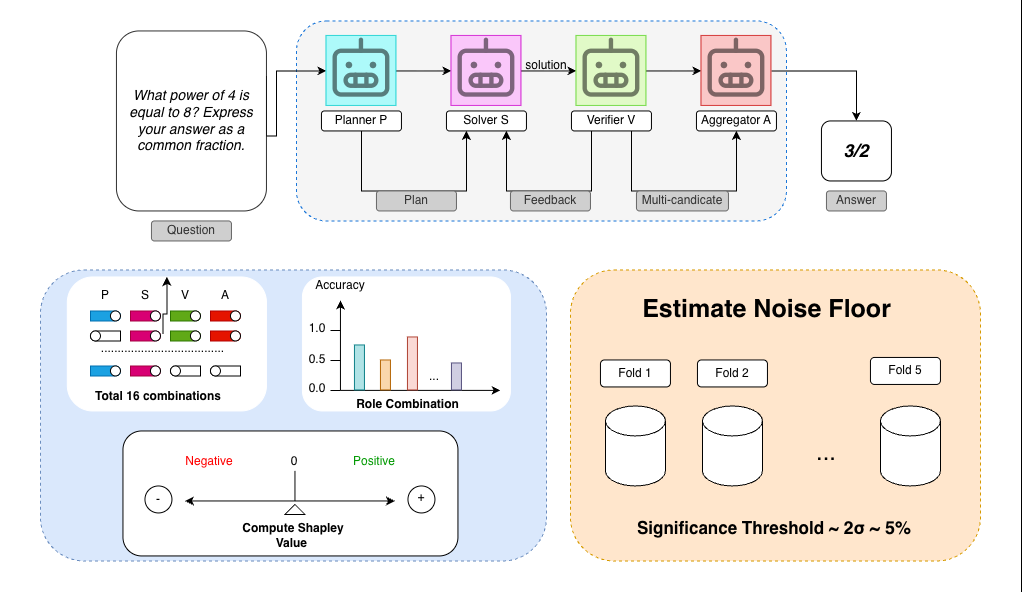
\includegraphics[width=\textwidth, height=0.68\textheight, keepaspectratio]{figs/pipeline_shapley_overview.png}
    \end{column}
    
    \begin{column}{0.48\textwidth}
      \begin{block}{\textbf{Đánh giá 16 liên minh vai trò}}
        \begin{itemize}\small
          \item \textbf{Solver ($S$):} Đóng góp $>90\%$ tổng giá trị hệ thống. Năng lực của Solver quyết định trần hiệu năng.
          \item \textbf{Planner ($P$):} Đóng góp $\approx 0$ trên các tác vụ toán/code có cấu trúc (sinh kế hoạch không giúp ích).
          \item \textbf{Verifier ($V$):} Đóng góp phụ thuộc chặt chẽ vào độ chính xác của tín hiệu kiểm.
          \item \textbf{Aggregator ($A$):} Tổng hợp bằng LLM không vượt trội hơn Bỏ phiếu đa số cơ học ($+0{,}8$ đến $+8{,}0$).
        \end{itemize}
      \end{block}
    \end{column}
  \end{columns}
\end{frame}

\begin{frame}{4.2. Năng lực Verifier: Tín hiệu tất định vs LLM-as-a-Judge}
  \begin{columns}[t]
    \begin{column}{0.50\textwidth}
      \begin{block}{\textbf{Kiểm chứng tất định (Code Execution)}}
        \centering\footnotesize
        \begin{tabular}{lcccc}\toprule
          \textbf{Cấu hình} & \textbf{Greedy} & \textbf{\texttt{exec3}} & \textbf{Phá bài}\\\midrule
          HE 1.5B (Kaggle) & 0,5375 & \textbf{0,6000} & \textbf{0,0}\\
          HE 1.5B (5090)   & 0,5625 & \textbf{0,6438} & \textbf{0,0}\\
          HE 7B (5090)     & 0,8000 & \textbf{0,8812} & \textbf{0,0}\\
          HE 7B (Kaggle)   & 0,7938 & \textbf{0,9000} & \textbf{0,0}\\\bottomrule
        \end{tabular}
        \vspace{4pt}
        \begin{itemize}\scriptsize
          \item Đạt đúng trần \textbf{Oracle@4}, phá $0$ bài trong 20/20 fold.
          \item Mức tăng $+6{,}3$ đến $+10{,}6$ điểm ròng so với baseline.
        \end{itemize}
      \end{block}
    \end{column}
    
    \begin{column}{0.46\textwidth}
      \begin{alertblock}{\textbf{Tín hiệu học được (LLM-as-a-Judge)}}
        \begin{itemize}\small
          \item Bộ phân loại trên HumanEval (\texttt{llm3}): Phá $2{,}6 - 4{,}6$ bài/fold.
          \item Độ chính xác thực tế tụt dưới mức greedy baseline.
          \item Bị chặn trên bởi Majority Voting.
        \end{itemize}
      \end{alertblock}
      
      \begin{block}{\textbf{Quy luật bão hòa}}
        \begin{itemize}\small
          \item GSM8K 7B (Solver đạt $0{,}916$): Verifier gây \textbf{26 bài phá} vs \textbf{6 bài sửa}.
          \item $\implies$ Verifier không hoàn hảo sẽ làm hại khi Solver đã mạnh.
        \end{itemize}
      \end{block}
    \end{column}
  \end{columns}
\end{frame}

\begin{frame}{4.3. Huấn luyện tác tử \& Hiện tượng lối tắt hàm thưởng}
  \begin{columns}[c]
    \begin{column}{0.48\textwidth}
      \centering
      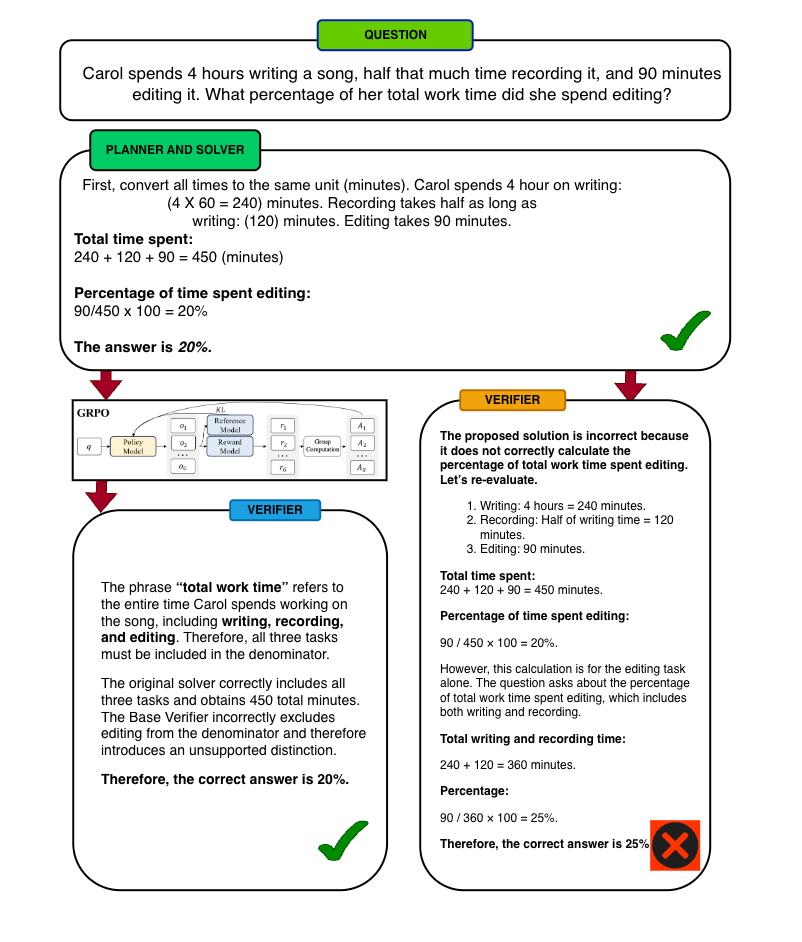
\includegraphics[width=\textwidth, height=0.68\textheight, keepaspectratio]{figs/verifier_grpo_example.png}
    \end{column}
    
    \begin{column}{0.48\textwidth}
      \begin{alertblock}{\textbf{Thất bại của RL (GRPO, ORPO, MAPoRL)}}
        \begin{itemize}\small
          \item 7 thử nghiệm huấn luyện đều không vượt qua được kiểm chứng đối chứng nghiêm ngặt.
          \item \textbf{Hiện tượng Reward Hacking (Lối tắt):}
            \begin{itemize}\footnotesize
              \item \textbf{Verifier:} Học cách luôn im lặng hoặc nhại lại đáp án của Solver để tối đa hóa reward an toàn.
              \item \textbf{Planner:} Học cách sinh plan rỗng để tránh bị trừ điểm độ dài.
            \end{itemize}
        \end{itemize}
      \end{alertblock}
      
      \begin{block}{\textbf{Kết luận kỹ thuật}}
        \small Mô hình tối ưu hóa hàm thưởng bằng cách "lách luật" bề mặt thay vì thực sự học khả năng suy luận logic.
      \end{block}
    \end{column}
  \end{columns}
\end{frame}

% =====================================================================
% PHAN V: CO CHE MOC THAM CHIEU & THIET KE
% =====================================================================
\section{Phần V: Cơ chế mốc tham chiếu \& Thiết kế}

\begin{frame}{5.1. Tác động của mốc tham chiếu \& Khoảng cách năng lực}
  \begin{columns}[c]
    \begin{column}{0.58\textwidth}
      \begin{tikzpicture}[scale=0.82, transform shape]
        \draw[->, thick, black!75] (0,0) -- (5.8,0) node[right, font=\scriptsize\bfseries] {Chênh lệch năng lực};
        \draw[->, thick, black!75] (0,-2.2) -- (0,2.5) node[above, font=\scriptsize\bfseries] {Hiệu ứng ròng (điểm)};
        
        \fill[LightBlueBg, opacity=0.7] (0,0) rectangle (1.7,2.2);
        \fill[LightRedBg, opacity=0.7] (1.7,-2.0) rectangle (5.5,0);
        
        % Duong so voi W
        \draw[very thick, BlueAccent] (0,0.5) -- (4.8,2.2);
        \fill[BlueAccent] (4.8,2.2) circle (2pt) node[above, font=\scriptsize\bfseries] {$+14{,}0$ (so với $W$)};
        
        % Duong so voi I
        \draw[very thick, CrimsonRed, dashed] (0,0.4) -- (5.2,-1.4);
        \fill[CrimsonRed] (4.8,-1.2) circle (2pt) node[below, font=\scriptsize\bfseries] {$-12{,}4$ (so với $I$)};
        
        % Nguong g*
        \draw[thick, gray, dotted] (1.7,-2.0) -- (1.7,2.2);
        \node[fill=white, draw=gray, rounded corners=2pt, font=\tiny\bfseries, inner sep=2pt] at (1.7,2.3) {Ngưỡng $g^* \approx 0{,}09$};
        
        \node[font=\tiny\itshape, text=BlueAccent] at (0.8,1.2) {Vùng $\dceil > 0$};
        \node[font=\tiny\itshape, text=CrimsonRed] at (3.5,-0.6) {Vùng $\dceil < 0$ (Suy giảm ròng)};
      \end{tikzpicture}
    \end{column}
    
    \begin{column}{0.40\textwidth}
      \begin{block}{\textbf{Cơ chế đảo chiều hiệu ứng}}
        \begin{itemize}\small
          \item \textbf{So với $W$:} Hiệu ứng luôn dương và tăng mạnh khi chênh lệch lớn (do năng lực của mô hình mạnh).
          \item \textbf{So với $I$:} Trần $\dceil$ giảm nhanh và âm khi vượt ngưỡng $g^* \approx 0{,}09$.
        \end{itemize}
      \end{block}
      
      \begin{alertblock}{\textbf{Quy luật tổn thất}}
        \centering\small
        Khi khoảng cách năng lực lớn (MATH):\\
        \textbf{Tổn thất $L \approx 11 \times$ Cơ hội $G$!}
      \end{alertblock}
    \end{column}
  \end{columns}
\end{frame}

\begin{frame}{5.2. Khuyến nghị thiết kế hệ thống thực tế}
  \begin{columns}[t]
    \begin{column}{0.48\textwidth}
      \begin{exampleblock}{\textbf{1. Miền có Kiểm chứng tất định (Code)}}
        \begin{itemize}\small
          \item \textbf{Chiến lược tối ưu:} Sampling độc lập từ cùng mô hình $+$ Lọc bằng Unit Test / Execution (\texttt{exec3}).
          \item \textbf{Hiệu quả:} Tiệm cận trần Oracle mà không làm hỏng bài đúng.
          \item Không cần thêm vai trò LLM Verifier phức tạp.
        \end{itemize}
      \end{exampleblock}
    \end{column}
    
    \begin{column}{0.48\textwidth}
      \begin{alertblock}{\textbf{2. Miền Suy luận mở (Toán, QA, Reasoning)}}
        \begin{itemize}\small
          \item \textbf{Chiến lược tối ưu:} Kích hoạt trực tiếp \textbf{Single Strong Model} hoặc Bỏ phiếu đa số cơ học.
          \item \textbf{Điều cấm kỵ:} Không chuyển giao artifact của mô hình nhỏ để mô hình lớn sửa.
          \item Tiết kiệm chi phí token và tránh tổn thất do thông tin sai lệch.
        \end{itemize}
      \end{alertblock}
    \end{column}
  \end{columns}
  
  \vspace{6pt}
  \begin{block}{\textbf{Đúc kết quy tắc triển khai}}
    \centering\small
    \emph{Tạo mẫu độc lập và tổng hợp khách quan luôn vượt trội hơn chuỗi sửa bài phụ thuộc.}
  \end{block}
\end{frame}

% =====================================================================
% PHAN VI: HAN CHE & TIEM NANG PHAT TRIEN
% =====================================================================
\section{Phần VI: Hạn chế \& Tiềm năng phát triển}

\begin{frame}{6.1. Hạn chế của nghiên cứu hiện tại}
  \begin{columns}[t]
    \begin{column}{0.48\textwidth}
      \begin{block}{\textbf{1. Phạm vi quy mô mô hình}}
        \begin{itemize}\small
          \item Nghiên cứu xác lập trên dải tham số từ \textbf{1,5B đến 32B}.
          \item Chưa kiểm chứng trực tiếp trên các mô hình ngôn ngữ quy mô siêu lớn ($>70\text{B}$).
        \end{itemize}
      \end{block}
      
      \begin{block}{\textbf{2. Chiến lược giải mã}}
        \begin{itemize}\small
          \item Nhánh luồng thông tin chủ yếu khảo sát giải mã tất định (\textbf{greedy decoding}).
          \item Chưa phân tầng triệt để theo nhiệt độ lấy mẫu (temperature sampling).
        \end{itemize}
      \end{block}
    \end{column}
    
    \begin{column}{0.48\textwidth}
      \begin{block}{\textbf{3. Mở rộng dữ liệu liên miền}}
        \begin{itemize}\small
          \item Phân tích chuyển dịch sang miền toán học mới dựa trên 3 cặp mô hình với khoảng tin cậy tương đối rộng.
          \item Ngưỡng đổi dấu $g^*$ cần gắn thêm khoảng tin cậy tham số mở rộng.
        \end{itemize}
      \end{block}
      
      \begin{block}{\textbf{4. Đánh giá gán công trạng}}
        \begin{itemize}\small
          \item Phân tích Shapley hiện dựa trên bootstrap theo mẫu bài toán mà chưa phân tích theo fold dữ liệu hoàn toàn độc lập.
        \end{itemize}
      \end{block}
    \end{column}
  \end{columns}
\end{frame}

\begin{frame}{6.2. Tiềm năng phát triển \& Hướng nghiên cứu tương lai}
  \begin{columns}[t]
    \begin{column}{0.48\textwidth}
      \begin{exampleblock}{\textbf{1. Kiến trúc Hybrid Verifier}}
        \begin{itemize}\small
          \item Kết hợp kiểm chứng thực thi tất định với các mô hình phần thưởng tiến trình (\textbf{Process Reward Models - PRM}).
          \item Giám sát và chấm điểm suy luận theo từng bước thay vì chỉ đánh giá đáp án cuối cùng.
        \end{itemize}
      \end{exampleblock}
      
      \begin{exampleblock}{\textbf{2. Định tuyến động (Dynamic Routing)}}
        \begin{itemize}\small
          \item Tự động ước lượng độ khó bài toán và khoảng cách năng lực thời gian thực.
          \item Chỉ kích hoạt multi-agent khi bài toán nằm trong "vùng can thiệp" khả thi.
        \end{itemize}
      \end{exampleblock}
    \end{column}
    
    \begin{column}{0.48\textwidth}
      \begin{exampleblock}{\textbf{3. Thiết kế hàm thưởng RL chống lối tắt}}
        \begin{itemize}\small
          \item Xây dựng hàm thưởng phạt thông tin dư thừa hoặc nhại lại lời giải (Information-theoretic penalties).
          \item Áp dụng cơ chế kiểm tra chéo độc lập giữa các tác tử trong quá trình cập nhật gradient.
        \end{itemize}
      \end{exampleblock}
      
      \begin{block}{\textbf{4. Mở rộng tác vụ dài hạn (Long-horizon)}}
        \begin{itemize}\small
          \item Mở rộng khung đo lường sang các bài toán phần mềm thực tế (SWE-bench, WebAgent).
        \end{itemize}
      \end{block}
    \end{column}
  \end{columns}
\end{frame}

% =====================================================================
% TONG KET & LOI CAM ON
% =====================================================================
\begin{frame}{Tổng kết bài học kỹ thuật cốt lõi}
  \begin{columns}[c]
    \begin{column}{0.95\textwidth}
      \begin{block}{\textbf{Ba kết luận kỹ thuật then chốt}}
        \begin{enumerate}\normalsize
          \item[\textbf{1.}] \textbf{Phối hợp đa tác tử không mặc định tốt hơn mô hình đơn lẻ:}\\
          Mức tăng biểu kiến chủ yếu xuất phát từ việc so với mô hình yếu. Khi so với mô hình mạnh ở cùng chi phí tính toán, đa tác tử thường hòa hoặc thua.
          \vspace{4pt}
          
          \item[\textbf{2.}] \textbf{Tổn thất do tiếp xúc thông tin sai lệch là rủi ro lớn nhất:}\\
          Mô hình mạnh bị suy giảm nghiêm trọng khi tiếp xúc artifact sai ($46{,}4\% \to 19{,}2\%$). Giao thức sửa bài hoạt động như kênh truyền dẫn hơn là cơ chế tự sửa lỗi.
          \vspace{4pt}
          
          \item[\textbf{3.}] \textbf{Tín hiệu kiểm chứng tất định là chìa khóa duy nhất:}\\
          Thực thi mã kiểm thử tiệm cận trần Oracle và triệt tiêu tổn thất ($L=0$), trong khi các bộ kiểm học được (LLM-as-a-judge) dễ phá bài và gặp hiện tượng lối tắt hàm thưởng.
        \end{enumerate}
      \end{block}
    \end{column}
  \end{columns}
\end{frame}

\begin{frame}[plain]
  \begin{tikzpicture}[remember picture,overlay]
    \fill[NavyMain] (current page.north west) rectangle (current page.south east);
  \end{tikzpicture}
  
  \centering
  \color{white}
  \vspace{0.6cm}
  {\Huge\bfseries LỜI CẢM ƠN}\\[8pt]
  {\color{AmberGold}\rule{0.3\linewidth}{1.2pt}}\\[14pt]
  
  \begin{minipage}{0.85\textwidth}
    \centering\normalsize
    Nhóm chúng em xin bày tỏ lòng biết ơn chân thành và sâu sắc nhất tới\\[6pt]
    {\Large\bfseries TS. Trần Hồng Việt}\\[4pt]
    \textit{Giảng viên phụ trách môn học Xử lý ngôn ngữ tự nhiên}\\[2pt]
    \textit{Viện Trí tuệ Nhân tạo --- Trường Đại học Công nghệ, ĐHQGHN}\\[12pt]
    
    \small
    Cảm ơn Thầy đã luôn tận tâm giảng dạy, truyền cảm hứng và định hướng phương pháp luận khoa học nghiêm cẩn trong suốt học kỳ vừa qua.
  \end{minipage}
  
  \vspace{1.0cm}
  {\Large\bfseries Q \& A}\\[4pt]
  {\small Kính mời Thầy và các bạn đặt câu hỏi thảo luận!}
\end{frame}

\end{document}
